\chapter{CFX Pre}
\label{ch:pre}

%-----------------------------------------------------------------------------------------------------------------
\section{Nomenclature}
\label{sec:nomenclature}

All models in foregoing section will use the following naming convention.
\begin{itemize}
	\item \textit{Reference:} no angle $\theta_{ref}=0^{\circ}$ 
	\item \textit{Model 1:} CCW angle $\theta_1=-20^{\circ}$ 
	\item \textit{Model 2:} CW angle $\theta_2=10^{\circ}$
\end{itemize}

The dimensionless coordinate system in $X,Y,Z$ directions \ref{eq:xstr} - \ref{eq:zstr} as per \cite{art}.
\begin{equation}
	X^* \equiv
	\begin{cases}
		\frac{X}{H}   & X\geq 0 \\
		\frac{X}{L_d} & X < 0   \\
	\end{cases}
	\label{eq:xstr}
\end{equation}
\begin{equation}
	\label{eq:ystr}
	Y^* \equiv \frac{Y}{H/2}
\end{equation}
\begin{equation}
	\label{eq:zstr}
	Z^* \equiv \frac{Z}{Z_c /2}
\end{equation}

Revelant apparatus parameters and findings from \cite{art} are summarized below in Table~\ref{tab:param}.
\begin{table}[H]
	\centering
	\caption[Project parameters.]{Project parameters.\cite{art}}
	\begin{tabular}{lccc}
		\toprule
		\textbf{Description}      & \textbf{Symbol} & \textbf{Value} & \textbf{Unit} \\
		\midrule
		Combustor height          & $H$             & 30             & mm            \\
		Dome height               & $L_d$           & 15             & mm            \\
		Bulk mean velocity        & $U_{REF}$       & 23.9           & m/s           \\
		Reynolds number           & $Re$            & 4.56E+04       & -             \\
		Width of side inlet       & $W_a$           & 15             & mm            \\
		Width of axial inlet      & $W_f$           & 1.58           & mm            \\
		Combustor span-wise width & $Z_c$           & 120            & mm            \\
		Duct length               & $L$             & 2000           & mm            \\
		\bottomrule
	\end{tabular}
	\label{tab:param}
\end{table}

%-----------------------------------------------------------------------------------------------------------------
\section{Mesh Specifications}
\label{sec:pre_mesh}

Using parameters from Table~\ref{tab:param} and \cite{projfaq}, a model of the combustors geometry is created with \cite{sld}. From this, selection of the computational domain is shown graphically (see Figure~\ref{fig:domain}).
\begin{figure}[H]
	\centering
	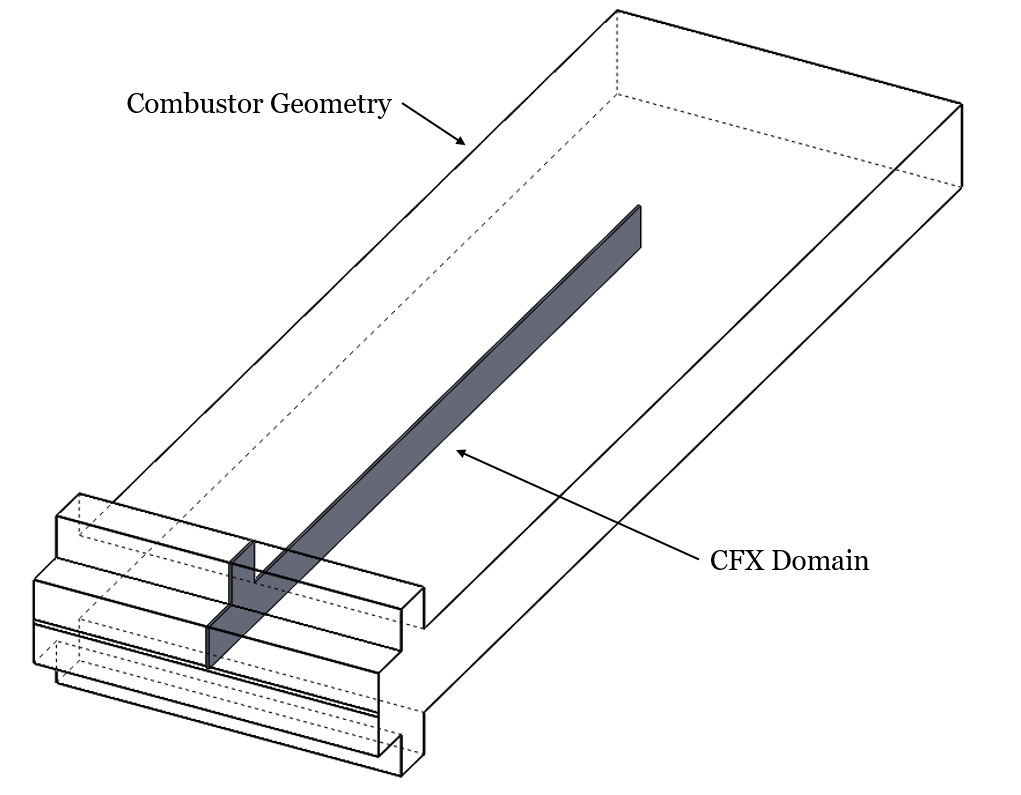
\includegraphics[width=0.75\textwidth]{ref/domain}
	\caption[Computational domain used in CFX simulations.]{Computational domain used in CFX simulations. \cite{sld}}
	\label{fig:domain}
\end{figure}

Note the CFX domain is modelled as for $X^* \in [-1,9]$ based on the required length for full flow development \cite{art}.\\


For all three models, an all triangular sweep mesh of maximum element size 0.001 [m] or 1 [mm] is used. In addition all domain wall boundaries were inflate 5 layers with a growth rate of 1.3 and maximum thickness of 0.001 [m] or 1 [mm] (see Figure~\ref{fig:inflation}.
\begin{figure}[H]
	\centering
	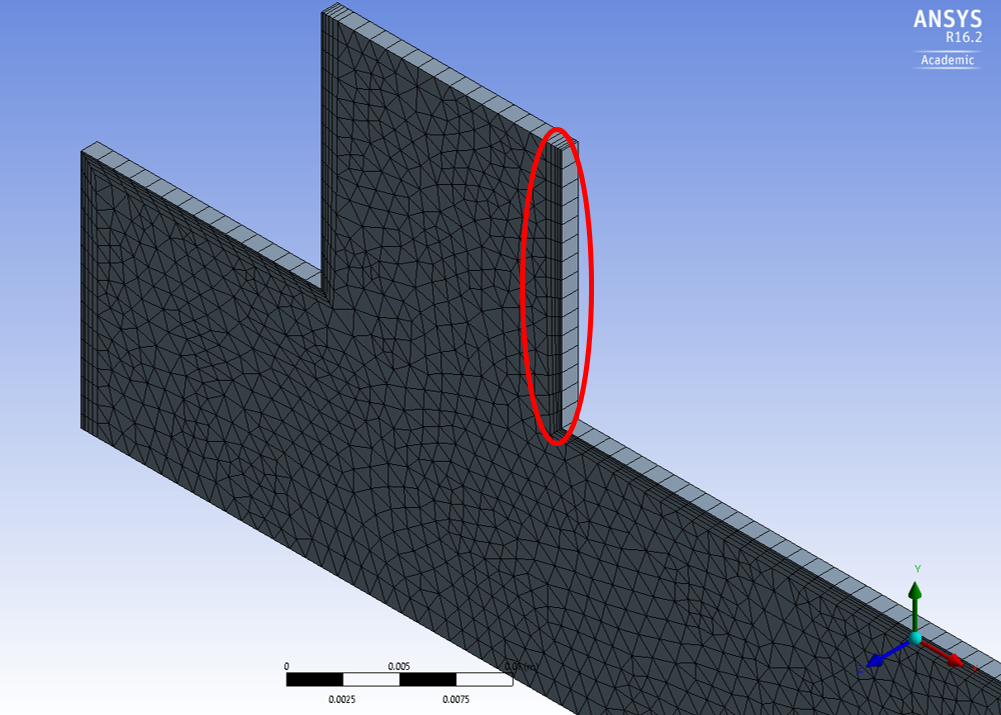
\includegraphics[width=0.75\textwidth]{ref/inflation}
	\caption[Final mesh with boundary layer inflation.]{Final mesh with boundary layer inflation.\cite{cfx}}
	\label{fig:inflation}
\end{figure}

Resulting a node count of $n_{ref}= 12398, n_1= 12418, n_2=11738$ for reference, first and second models respectively.\\

See Section~\ref{sec:pre_summary} for all meshes used in CFX simulations.

\textbf{Justification.}
%-----------------------------------------------------------------------------------------------------------------
\section{Boundary Conditions}
\label{sec:pre_bc}

Axial inlet conditions were set to be constant throughout all models. The $X^*=-1$ face is split to model the inlet's rectangular face of height $W_f/2=0.79$ [mm]. Assuming subsonic and steady conditions, the input velocity is $u=92.73$ [m/s] \cite{projfaq} at a temperature of $T=100 ^{\circ}$C. Temperature is used as a passive fluid marker to simulate the mixing of fuel. A turbulent kinetic energy (KE) of $I=13.6$ \% with an auto computed turbulent length scale \cite{projfaq}.\\

Side inlets were also considered to be subsonic. A fractional turbulent KE of $I=1.03$ \%, again with an auto computed turbulent length scale \cite{projfaq}. Due to the varying inlet angle $\theta$, the measured normal entrance velocity must be decomposed into respective $u-v$ Cartesian coordinates. Based on the measured -19.74 [m/s] on the $Y^*=2$ face at $X^*=0.25$, $u-v$ assigned side inlet velocities are calculated as seen below in Table~\ref{tab:sideinletbc}.
\begin{table}[H]
	\centering
	\caption{Side inlet velocities for each model.}
	\begin{tabular}{cccc}
		\toprule		
		\multicolumn{1}{c}{} & \textbf{Ref.} & \textbf{Model 1} & \textbf{ Model 2} \\
		\midrule
		$\theta_i$	& 0            & -20             & 10		\\
		$u$			& 0            & 6.75            & -3.43	\\
		$v$ 		& -19.74       & -18.55          & -19.44	\\
		\bottomrule
	\end{tabular}
	\label{tab:sideinletbc}
\end{table}
The side inlet's temperature is assigned to be $T=0 ^{\circ}$C to simulate an air mixture without fuel.

All models have a subsonic and steady outlet at the $X^*=9$ face. A static pressure of $P=0$ [Pa] is assigned to the outlet.\\

To save computational resources, the symmetry boundary condition is applied the $Y^*=0$ face. The same boundary condition is also applied to both faces in the $Z$ direction. This is done to ignore the side wall effects and reduce this complex 3D problem to a simple two dimensional one (i.e. no variation in $Z$).\\

All other faces were assigned a smooth and adiabatic no-slip wall condition. \\

See Section~\ref{sec:pre_summary} for graphical summaries of all boundary conditions used CFX simulations.
%-----------------------------------------------------------------------------------------------------------------
\section{Fluid Properties}
\label{sec:pre_fluid}

The entire CFX domain is assigned a continuous ideal gas air due to the temperature variation which will cause a change in density $\rho$. The domain is also assigned to be ``Stationary'' and ``Non Buoyant''.\\

The heat transfer model is set to ``Thermal Energy'' because the flow is incompressible  therefore significant velocity effects do not need to be included \cite{tut}. The Mach number Ma is calculated as \ref{eq:ma} \cite{fluids}.
\begin{equation}
	\label{eq:ma}
	 \text{Ma}\equiv \frac{U}{a} 
\end{equation}

Where $a=343$ [m/s] is the speed of sound. Since Ma = $\tfrac{92.73}{343}=0.3 \leq 1$, the flow is not compressible.\\

\textbf{Applicability of $k-\varepsilon$ Model.}

\textbf{Justification.}

%-----------------------------------------------------------------------------------------------------------------
\section{Numerical Parameters}
\label{sec:pre_num}

High resolution advection scheme and turbulence metrics.\\

For good results \cite{tut}, the following equation is used to calculate the physical timescale $t_s$. 
\begin{equation}
	\label{eq:ts}
	t_s = \frac{1}{3} \left( \frac{L}{U} \right)
\end{equation}
Using $L = L_d + X^* H = 285$ [mm] = 0.285 [m] $\Rightarrow t_s$ 0.004 [s].\\  

With a maximum iteration count of 50, the maximum residuals $\delta_{r_{MAX}}$ is set to 0.0001 for accurate results.

%-----------------------------------------------------------------------------------------------------------------
\section{Model Summary}
\label{sec:pre_summary}

Summaries for all models are shown in Figures~\ref{fig:ref_modsum}, \ref{fig:mod1_modsum},  \ref{fig:mod2_modsum} on the following pages.

\begin{figure}[H]
	\centering
	\includegraphics[height=0.95\textheight,keepaspectratio]{ref/model_summary}
	\caption{Reference model CFX-Pre summary.}
	\label{fig:ref_modsum}
\end{figure}
\begin{figure}[H]
	\centering
	\includegraphics[height=0.95\textheight,keepaspectratio]{model1/model_summary}
	\caption{Model 1 CFX-Pre summary.}
	\label{fig:mod1_modsum}
\end{figure}
\begin{figure}[H]
	\centering
	\includegraphics[height=0.95\textheight,keepaspectratio]{model2/model_summary}
	\caption{Model 2 CFX-Pre summary.}
	\label{fig:mod2_modsum}
\end{figure}